%% 《高级图论》课程论文 V3
%% 基于《计算机学报》单栏 CjC 模板（Overleaf: latextemplet-CjC-xelatex）
%% 编译方式：XeLaTeX；请将本文件与 figures/、ref.bib 放入模板工程后编译
\documentclass[10.5pt,compsoc,UTF8]{CjC}
\usepackage{CTEX}
\usepackage{graphicx}
\usepackage{footmisc}
\usepackage{subfigure}
\usepackage{url}
\usepackage{multirow}
\usepackage{multicol}
\usepackage[noadjust]{cite}
\usepackage{amsmath,amsthm}
\usepackage{amssymb,amsfonts}
\usepackage{booktabs}
\usepackage{color}
\usepackage{ccaption}
\usepackage{float}
\usepackage{fancyhdr}
\usepackage{caption}
\usepackage{algorithm}
\usepackage{algpseudocode}
\usepackage{xcolor,stfloats}
\usepackage{comment}
\setcounter{page}{1}
\graphicspath{{figures/}}
\usepackage{cuted}
\usepackage{captionhack}
\usepackage{epstopdf}
\usepackage{gbt7714}

%===============================%
\headevenname{\mbox{\quad} \hfill  \mbox{\zihao{-5}{ \hfill 《高级图论》课程论文  } \hspace {50mm} \mbox{2026 年 7 月}}}%
\headoddname{杜浩存 \hfill 面向数据推断泄露的任意字段集合敏感度评估图 oracle}%

\renewcommand{\thefootnote}{\fnsymbol{footnote}}
\setcounter{footnote}{0}
\renewcommand\footnotelayout{\zihao{5-}}

\newtheoremstyle{mystyle}{6pt}{6pt}{\normalfont}{1em}{\bf}{}{1em}{}
\theoremstyle{mystyle}
\newtheorem{definition}{定义}
\newtheorem{observation}{观察}
\renewcommand\figurename{图~}
\renewcommand{\thesubfigure}{(\alph{subfigure})}
\newcommand{\upcite}[1]{\textsuperscript{\cite{#1}}}
\renewcommand{\labelenumi}{(\arabic{enumi})}
\newcommand{\tabincell}[2]{\begin{tabular}{@{}#1@{}}#2\end{tabular}}
\renewcommand{\bibsection}{}
\makeatletter
\renewcommand{\@biblabel}[1]{[#1]\hfill}
\makeatother
\setlength\parindent{2em}

\begin{document}

\hyphenpenalty=50000
\thispagestyle{plain}%
\thispagestyle{empty}%
\pagestyle{CjCheadings}

\vspace {-13mm}
\onecolumn
\zihao{5-}\noindent 杜浩存 \hfill 《高级图论》课程论文\hfill 2026 年 7 月\\
\noindent\rule[0.25\baselineskip]{\textwidth}{1pt}

{
\centering
\vspace {11mm}
{\zihao{2} \heiti 面向数据推断泄露的任意字段集合\\敏感度评估图 oracle}

\vskip 5mm

{\zihao{4}\fangsong 杜浩存}

\vspace {5mm}

\zihao{5}{(西安交通大学\quad 西安\quad 710049)}
}

\vskip 5mm

\zihao{5}{
\setlength{\baselineskip}{16pt}\selectfont{
\noindent {\heiti 摘\quad 要\quad }
电网运行数据在共享前通常仅删除机密字段，但保留字段之间由物理定律与统计规律决定的耦合，使攻击者仍能训练推断模型间接恢复机密量，即数据推断泄露。本文指出，泄露风险本质上是可见字段\textbf{集合}上的集合函数 $v_c(S)$，而非单字段属性——存在大量“单看安全、合体泄露”的组合，例如风电出力与风电占比单独推断总发电量的测试 $R^2$ 仅 0.064 与 0.162，合体后升至 0.928。忠实评估 $v_c(S)$ 要求对每个集合重训攻击者以刻画“攻击者最优响应”，但 44 个字段的可见集合多达 $2^{44}$ 个，逐集合重训不可行。本文的核心贡献是提出一个\textbf{子集条件图 oracle}：以字段相关图为骨架，采用可见性感知的注意力消息传递，通过随机子集失活方式一次性训练，即可对任意可见集合以单次前向给出敏感度估计；再以 $K$ 步查询时微调闭合摊销残差。该 oracle 将单集合评估成本由一次完整重训（分钟级）降至秒级：在 1431 个字段集合、17172 条逐机密字段真值上，微调 200 步后估计对重训真值的平均绝对误差为 0.039、排序 Spearman 相关系数达 0.95，每集合仅约 3 秒。基于该 oracle，本文进一步提出“全扫描 + 重训认证”协议以低成本发现协同泄露：在 $\binom{44}{2}=946$ 个字段对上构建二阶协同图，在 $\binom{44}{3}=13244$ 个三元组上定位真不可约三阶协同。实验发现最强二阶协同“风电出力 + 风电占比 $\to$ 总发电量”达 0.765，最强三阶协同“燃气出力 + 燃气占比 + 负荷预测 $\to$ 净交换功率”达 0.455；估计与认证排序相关 0.795 且估计系统性保守，随机对照组阳性率仅 19/2400，证明高阶协同是稀疏且物理可解释的结构。消融实验表明，图结构相较多层感知机在 5 字段以上集合的专用推断上具一致精度优势，且其参数与字段身份解耦，具备跨系统迁移潜力；此外基于置零的评估口径相对重训真值系统性低估协同 3.4 倍、排序相关仅 0.351，表明忠实评估必须以重训为真值。
\par}}
\vspace {5mm}

\zihao{5}{\noindent
{\heiti 关键词 \quad }图神经网络；集合函数；数据推断泄露；子集条件模型；协同效应；数据脱敏
}

\vskip 7mm

\begin{center}
\zihao{3}{ \heiti A Graph Oracle for Sensitivity Assessment of Arbitrary Field Subsets against Data Inference Leakage}\\
\vspace {5mm}
\zihao{5}{ DU Hao-Cun}\\
\vspace {2mm}
\zihao{5-}{{(Xi'an Jiaotong University, Xi'an 710049, China)}}
\end{center}

\zihao{5}{
\setlength{\baselineskip}{18pt}\selectfont{
{\bf Abstract}\quad
Operational power grid data are usually desensitized by simply removing confidential fields before sharing, yet the physical and statistical couplings among the remaining fields still allow an attacker to train inference models and indirectly recover confidential quantities --- a threat known as data inference leakage (DIL). This paper argues that leakage risk is essentially a set function $v_c(S)$ over subsets of visible fields, rather than a property of individual fields: many combinations are ``individually harmless yet jointly revealing'', e.g., wind generation (MW) and wind share individually infer total generation with test $R^2$ of only 0.064 and 0.162, but jointly reach 0.928. Faithfully evaluating $v_c(S)$ requires retraining an attacker for each subset to capture the ``attacker's best response'', but the $2^{44}$ possible visible subsets over 44 fields make per-subset retraining intractable. The core contribution of this paper is a \textbf{subset-conditional graph oracle}: built upon a field correlation graph with visibility-aware attention message passing, it is trained once via random subset dropout and estimates the sensitivity of any visible subset in a single forward pass; a $K$-step query-time fine-tuning then closes the amortization gap. The oracle reduces the per-subset evaluation cost from a full retraining (minutes) to seconds: on 1431 field subsets and 17172 per-confidential-field ground-truth entries, after 200 fine-tuning steps its estimates achieve a mean absolute error of 0.039 and a ranking Spearman correlation of 0.95 against retraining truth, at about 3 seconds per subset. Based on this oracle, a ``scan-then-certify'' protocol is proposed to discover synergistic leakage cheaply: a second-order synergy graph is built over all $\binom{44}{2}=946$ field pairs, and irreducible third-order synergies are located among all $\binom{44}{3}=13244$ triples. The strongest second-order synergy ``wind MW + wind share $\to$ total generation'' reaches 0.765 and the strongest third-order synergy ``gas MW + gas share + load forecast $\to$ net interchange'' reaches 0.455; estimated and certified rankings correlate at 0.795 with the estimator being systematically conservative, and the random control group has a positive rate of only 19/2400, showing that higher-order synergies form a sparse and physically interpretable structure. Ablations show that the graph structure consistently outperforms an MLP on dedicated inference over subsets with five or more fields and that its parameters are decoupled from field identities, indicating cross-system transfer potential; moreover, a zeroing-based assessment underestimates synergy by 3.4 times with a rank correlation of merely 0.351 against retraining truth, indicating that faithful assessment must be grounded in retraining.
\par}}
\vspace {5mm}

{{\bf Keywords}\quad graph neural network; set function; data inference leakage; subset-conditional model; synergy; data desensitization\par}

\zihao{5}
\vskip 10mm

%%%%%%%%%%%%%%%%%%%%%%%%%%%%%%%%%%%%%%%%%%
\section{\heiti 引言}

现代电力系统已演化为深度互联的信息物理系统，其调度、市场与规划高度依赖细粒度运行数据在多主体间的持续共享。共享前的脱敏在工程实践中往往被简化为“删除机密字段”这一步，但保留下来的一般字段之间存在由物理定律（潮流方程、功率平衡、燃料—出力关系）与统计规律（负荷周期性、气象相关性、市场联动）共同决定的强耦合，攻击者完全可以用公开字段训练推断模型，间接恢复被删除的机密量。这一威胁被称为数据推断泄露（Data Inference Leakage, DIL）\upcite{hu2026ignn}。真实事件已反复印证其危害：看似无害的聚合运动数据曾暴露军事基地布局，而 2015 年乌克兰电网攻击的长期侦察阶段，攻击者正是借低敏感度的系统日志逐步推断出 SCADA 拓扑与操作逻辑。不评估推断泄露就共享“低敏感”数据，可能暴露系统中最关键的信息。

面向该威胁的代表性工作 IGNN\upcite{hu2026ignn} 构建字段间推断关系图，用图注意力网络为\textbf{每个字段}输出一个标量敏感度分数。然而本文观察到，以“单字段分数”刻画泄露存在原理性缺陷：\textbf{泄露不是字段的属性，而是字段集合的属性}。一个动机实例最为直观（完整数据见表 2）——风电出力（MW）与风电占比两个字段，各自单独推断机密字段“总发电量”的测试 $R^2$ 分别仅 0.064 与 0.162，按任何单字段评分都属低风险；但两者同时可见时 $R^2$ 跃升至 0.928，因为总发电量在物理上恰等于出力除以占比。更极端地，太阳能出力单独推断的 $R^2$ 仅 0.006（几乎无泄露），却参与增量达 0.596 的协同泄露。单字段分数在原理上无法同时刻画“太阳能出力单独共享安全”与“其与占比合体高危”这两个事实。因此，敏感度评估必须升维为定义在\textbf{任意字段集合}上的集合函数。

升维之后的根本困难在于\textbf{评估}。“集合 $S$ 的敏感度”应刻画攻击者拿到 $S$ 后所能达到的推断能力上限，即允许攻击者针对 $S$ 从头重训至最优的“最优响应”语义；而以固定模型加特征置零来近似（IGNN 与多数特征归因方法的做法）会产生分布外伪影，本文实验证明该口径系统性低估协同 3.4 倍。但忠实的重训语义带来沉重代价：$n=44$ 个字段的可见集合多达 $2^{44}\approx1.8\times10^{13}$ 个，而单次重训即需分钟级开销，逐集合枚举在计算上绝无可能。\textbf{如何以远低于逐点重训的成本，忠实评估任意集合的敏感度}，是本文要解决的核心问题。

本文的核心答案是一个\textbf{子集条件图 oracle}（图 1）。其关键思想是把“集合 $\mapsto$ 重训敏感度”这一映射\textbf{摊销}进单一模型：以字段相关图为骨架、采用可见性感知的注意力消息传递，通过随机子集失活方式一次性训练，使同一组参数学会对任意可见掩码给出条件推断；查询任意集合时只需一次前向即得估计，再以 $K$ 步查询时微调把通用表示快速特化到目标集合，闭合摊销残差。这样，单集合评估成本从一次完整重训（分钟级）降至秒级，而排序保真度足以支撑在指数空间中的检索。在此基础上，本文提出“全扫描 + 重训认证”协议，以廉价的 oracle 扫描组合空间、以昂贵但忠实的重训认证候选，二者构成“估计只用于筛选、结论以重训证书落地”的闭环，从而在 $\binom{44}{2}$ 与 $\binom{44}{3}$ 的空间里低成本地发现二阶协同图与三阶协同超图。

本文主要贡献如下：

(1) \textbf{问题与视角}。将数据推断泄露的敏感度评估从单字段分数升维为任意集合上的集合函数 $v_c(S)$，赋予其攻击者最优响应语义，并揭示单字段评分的原理性不适定性（第 3 节）。

(2) \textbf{方法（核心）}。提出子集条件图 oracle 及其可见性感知消息传递机制与随机子集失活训练，配合 $K$ 步查询时微调，实现任意集合敏感度的秒级忠实评估；并将其组织为“扫描—认证”协议以支撑高阶协同发现（第 4 节）。

(3) \textbf{系统实验}。在 PJM 真实数据的 1431 个字段集合、17172 条逐机密字段真值上，系统评估 oracle 的保真度（微调后 MAE 0.039、排序 Spearman 0.95）、成本（约 3 秒/集合）、逐规模行为与种子稳健性；给出图结构对多层感知机的消融、置零口径的定量否定，以及二/三阶协同的完整发现与认证（第 5 节）。

本文其余部分组织如下：第 2 节简述相关工作；第 3 节给出威胁模型与问题形式化；第 4 节详述方法；第 5 节展开系统实验；第 6 节讨论；第 7 节总结。

\section{\heiti 相关工作}

\textbf{数据敏感度评估}。IGNN\upcite{hu2026ignn} 将电网字段间推断关系组织为图并以图注意力网络输出字段级敏感度，是本文的直接对照。本文与其共享“用图组织字段关系”的思路，但在两点上根本不同：输出粒度从单字段分数升维为任意集合的集合函数，测量口径从“固定模型 + 风险传播”改为“逐集合重训的最优响应”，从而能够表达并忠实度量协同泄露。

\textbf{特征子集贡献与交互}。SHAP\upcite{lundberg2017shap} 及其摊销加速 FastSHAP\upcite{jethani2022fastshap}、ViT-Shapley\upcite{covert2023vitshapley} 研究固定模型下特征子集的边际贡献，Grabisch 等\upcite{grabisch1999interaction} 给出任意阶交互指标的公理化。这些方法刻画的是某个\textbf{固定模型}在特征扰动下的行为，本文的 $v_c(S)$ 则允许攻击者对每个 $S$ 重训至最优，刻画数据本身的可推断上限。两者“一个摊销模型回答所有子集查询”的思想相通，这也是本文 oracle 的方法学近亲；Datamodels\upcite{ilyas2022datamodels} 在训练数据维度拟合“子集 $\mapsto$ 性能”，与本文在特征维度的工作平行。

\textbf{任意条件建模与图学习}。VAEAC\upcite{ivanov2019vaeac}、ACFlow\upcite{li2020acflow} 学习任意观测子集条件化的生成模型，GRAPE\upcite{you2020grape} 将缺失特征学习建模为二部图上的表示学习；本文 oracle 在“随机掩码 + 联合训练”的机制上借鉴该族，但目标是集合函数的摊销而非数据分布。GCN\upcite{kipf2017gcn} 与 GAT\upcite{velickovic2018gat} 提供基础算子；Battaglia 等\upcite{battaglia2018relational} 与 Grinsztajn 等\upcite{grinsztajn2022tabular} 关于关系归纳偏置适用边界的论述，构成本文对图结构收益“按角色定位”的理论背景。

\section{\heiti 威胁模型与问题形式化}

\subsection{威胁模型}

设数据表含 $n$ 个字段 $F=\{f_1,\dots,f_n\}$（本文 $n=44$），其中规程认定的机密字段集为 $C\subset F$（本文 $|C|=12$，含总发电量、计量负荷、净交换功率、系统损耗、日前/实时阻塞价格及三类备用总量等），其余为一般字段集 $G=F\setminus C$。共享时机密字段被删除，攻击者获得某可见集合 $S\subseteq G$ 的完整列数据。假设攻击者拥有同分布历史对齐样本、知晓字段物理语义、且可从任意模型族训练推断模型（不受限于任何固定预训练模型）——这是对攻击者有利的保守假设，据此得到的是风险的上界刻画。防御方目标：对任意拟共享集合 $S$，在可接受成本内评估每个机密字段被推断的风险，并定位构成协同泄露的字段组合。

\subsection{作为集合函数的敏感度}

\begin{definition}[集合敏感度]
给定机密字段 $c\in C$ 与可见集合 $S\subseteq G$，集合敏感度为
\begin{equation}
v_c(S)=\max\Bigl(0,\ \sup_{g\in\mathcal{G}} R^2_{\mathrm{test}}\bigl(g(X_S);x_c\bigr)\Bigr),
\label{eq:vcs}
\end{equation}
其中 $X_S$ 为仅保留 $S$ 中字段的数据，$R^2_{\mathrm{test}}$ 为保留测试集上的决定系数。
\end{definition}

式 (\ref{eq:vcs}) 的上确界取在模型族与训练过程之上，即\textbf{攻击者最优响应}语义：对每个 $S$ 攻击者从头重训至最优。实践中以“在多种结构上分别重训并逐机密字段取较优”作为 $\sup$ 的经验近似。$v_c(\cdot)$ 是布尔格 $(2^{G},\subseteq)$ 上的集合函数，在最优响应语义下理论单调不减。对其 $2^{44}$ 个元素逐点重训不可行，这正是第 4 节 oracle 的动机。

\subsection{协同结构：协同图与协同超图}

\begin{definition}[$k$ 阶不可约协同]
字段对的二阶协同 $\mathrm{syn}_2^c(i,j)=v_c(\{i,j\})-\max(v_c(\{i\}),v_c(\{j\}))$；一般地，集合 $T$（$|T|=k\ge2$）的 $k$ 阶不可约协同为其相对最优 $(k{-}1)$ 阶子集的增量
\begin{equation}
\mathrm{syn}_k^c(T)=v_c(T)-\max_{T'\subset T,\,|T'|=k-1} v_c(T').
\label{eq:synk}
\end{equation}
\end{definition}

采用“减去最优低阶子集”而非全交互展开，源于安全语义：防御者关心“同时放行 $T$ 是否比放行其任何真子集更危险”，$\mathrm{syn}_k>0$ 直接回答该问题，且逐层定义天然支持递归剪枝（4.6 节）。以字段为顶点、$w(i,j)=\max_{c}\mathrm{syn}_2^c(i,j)$ 为边权得\textbf{协同图} $G_{\mathrm{syn}}=(F,E_2)$；显著三阶协同的三元组与 $F$ 构成 3 一致\textbf{协同超图} $H_{\mathrm{syn}}=(F,E_3)$。它们把泄露的组合结构组织为可分析的图论对象：如“删除最少字段使全部显著协同失效”即转化为其上的顶点覆盖类问题。

\subsection{测量口径与噪声底}

集合敏感度数值高度依赖口径。本文以\textbf{重训}为真值：对每个待测集合从头训练攻击者、实测 $R^2$。作为对照的\textbf{置零}口径（保持全字段模型 $g^{*}_F$ 参数不变、将 $S$ 外字段置零后测残余精度 $\tilde v_c(S)=\max(0,R^2_{\mathrm{test}}(g^{*}_F(X\odot m_S);x_c))$，$m_S$ 为 $S$ 的指示掩码）虽廉价，却因输入偏离训练分布、且固定参数无法表达针对 $S$ 的重新优化而系统性失真（5.4 节定量否定）。对同一集合以不同种子重复重训，实测复现噪声底 $\sigma\approx0.002$--$0.004$；据此设定判读标尺：单点差异 $>0.01$（多层感知机）/$>0.02$（图模型）方显著，协同显著阈值取 $\mathrm{syn}>0.10$（约噪声底 25 倍以上）。

\section{\heiti 方法}

\subsection{总览}

图 1 给出方法总览。系统以字段相关图为结构先验，其核心是\textbf{子集条件图 oracle}——一个把“任意可见集合 $\mapsto$ 重训敏感度”映射摊销进单一模型的估计器：训练时以随机子集失活遍历掩码空间（4.4 节），查询时一次前向加 $K$ 步微调即给出任意集合的秒级估计（4.3、4.5 节），并始终以逐集合重训真值校准。基于该 oracle，两类下游应用得以低成本实现：一是任意集合的直接敏感度查询（查表式风险评估），二是通过“扫描—认证”协议发现协同泄露（4.6 节）。贯穿全框架的设计原则是\textbf{估计层与真值层分离}：oracle 承担秒级、可扫描的筛选，重训承担忠实、可认证的定论，一切进入结论的数值都由重训产生。

\begin{figure}[htbp]
\centering
\centerline{
\includegraphics[width=0.99\linewidth]{framework_zh.png}}
{\heiti 图 1\quad 方法总览。以字段相关图为先验，子集条件图 oracle 一次训练后对任意可见集合秒级估计敏感度；下游支撑“任意集合直接评估”与“扫描—认证协同发现”两类应用；估计层与真值层分离}
\label{fig:framework}
\end{figure}

\subsection{字段相关图构建}

字段间推断关系既含线性相关，也含比值、饱和等非线性耦合。对每对字段 $(i,j)$ 计算五种相关性度量——Pearson、Spearman、Kendall 相关系数、归一化互信息与距离相关——并取绝对值平均得 $A_{\mathrm{raw}}(i,j)$。前三者捕获单调关联，后两者捕获一般非线性依赖，融合后对“占比—出力—总量”这类比值型物理关系保持敏感。以“阈值或 top-$k$”规则稀疏化得边集
\begin{equation}
E=\{(i,j):A_{\mathrm{raw}}(i,j)\ge\tau\}\cup\{(i,j):j\in\mathrm{top}\text{-}k_{\min}(i)\},
\label{eq:edge}
\end{equation}
本文取 $\tau=0.15$、$k_{\min}=8$ 并对称化。阈值项保证强关联入图，top-$k$ 项保证每个顶点的最小度以避免孤立点。需强调 $G$ 的定位：它是消息传递的\textbf{结构先验}而非因果图；协同泄露可能发生在两两相关都弱的字段间（如太阳能出力对），故框架不依赖 $G$ 的边权做任何敏感度结论，结论一律由重训产生。

\subsection{子集条件图 oracle}

oracle 以 $G$ 为骨架，把每个字段视为一个节点。其关键在于让\textbf{同一组参数}适配任意可见掩码 $m_S\in\{0,1\}^{n}$，机制如图 2 所示。

\textbf{输入编码}。节点 $i$ 的初始表示编码“观测值 $\times$ 可见位”与“可见位”二元组：
\begin{equation}
\mathbf{h}_i^{(0)}=\phi\bigl([\,x_i\cdot m_i;\ m_i\,]\bigr),
\label{eq:enc}
\end{equation}
$\phi$ 为共享编码器。显式输入 $m_i$ 使模型能区分“取值为零”与“不可见”，这是掩码条件化的前提。

\textbf{可见性感知注意力}。在第 $l$ 层，节点 $i$ 只从\textbf{可见}邻居聚合，注意力在可见邻居上重归一化：
\begin{equation}
\alpha_{ij}^{(l)}(m)=\frac{m_j\exp\bigl(\mathrm{score}^{(l)}(\mathbf{h}_i^{(l)},\mathbf{h}_j^{(l)})/T\bigr)}{\sum_{k\in\mathcal{N}(i)}m_k\exp\bigl(\mathrm{score}^{(l)}(\mathbf{h}_i^{(l)},\mathbf{h}_k^{(l)})/T\bigr)},
\label{eq:visatt}
\end{equation}
$T$ 为温度。与标准图注意力\upcite{velickovic2018gat}相比，掩码 $m_j$ 把不可见邻居从 softmax 分母中移除，使\textbf{同一组注意力参数在不同掩码下自动重新分配聚合权重}——这正是“一张图适配任意可见模式”的机制基础（图 2 中 $j_3,j_4$ 不可见故被移出聚合）。层间传播为
\begin{equation}
\mathbf{h}_i^{(l+1)}=\sigma\Bigl(\mathbf{W}_{\mathrm{self}}^{(l)}\mathbf{h}_i^{(l)}+\sum_{j\in\mathcal{N}(i)}\alpha_{ij}^{(l)}(m)\,\mathbf{W}_{\mathrm{neigh}}^{(l)}\mathbf{h}_j^{(l)}\Bigr),
\label{eq:layer}
\end{equation}
自环项 $\mathbf{W}_{\mathrm{self}}$ 保证可见节点自身信息不被邻居稀释。

\textbf{目标读出}。每个机密字段 $c$ 配可学习查询嵌入 $\mathbf{q}_c$，经 $L$ 层传播后以注意力读出，使不同机密目标聚焦不同的字段子图：
\begin{equation}
\hat{x}_c=\mathbf{w}_c^{\top}\sum_{i\in F}\mathrm{softmax}_i\bigl(\mathbf{q}_c^{\top}\mathbf{K}\mathbf{h}_i^{(L)}\bigr)\mathbf{h}_i^{(L)}.
\label{eq:readout}
\end{equation}

\begin{figure}[htbp]
\centering
\centerline{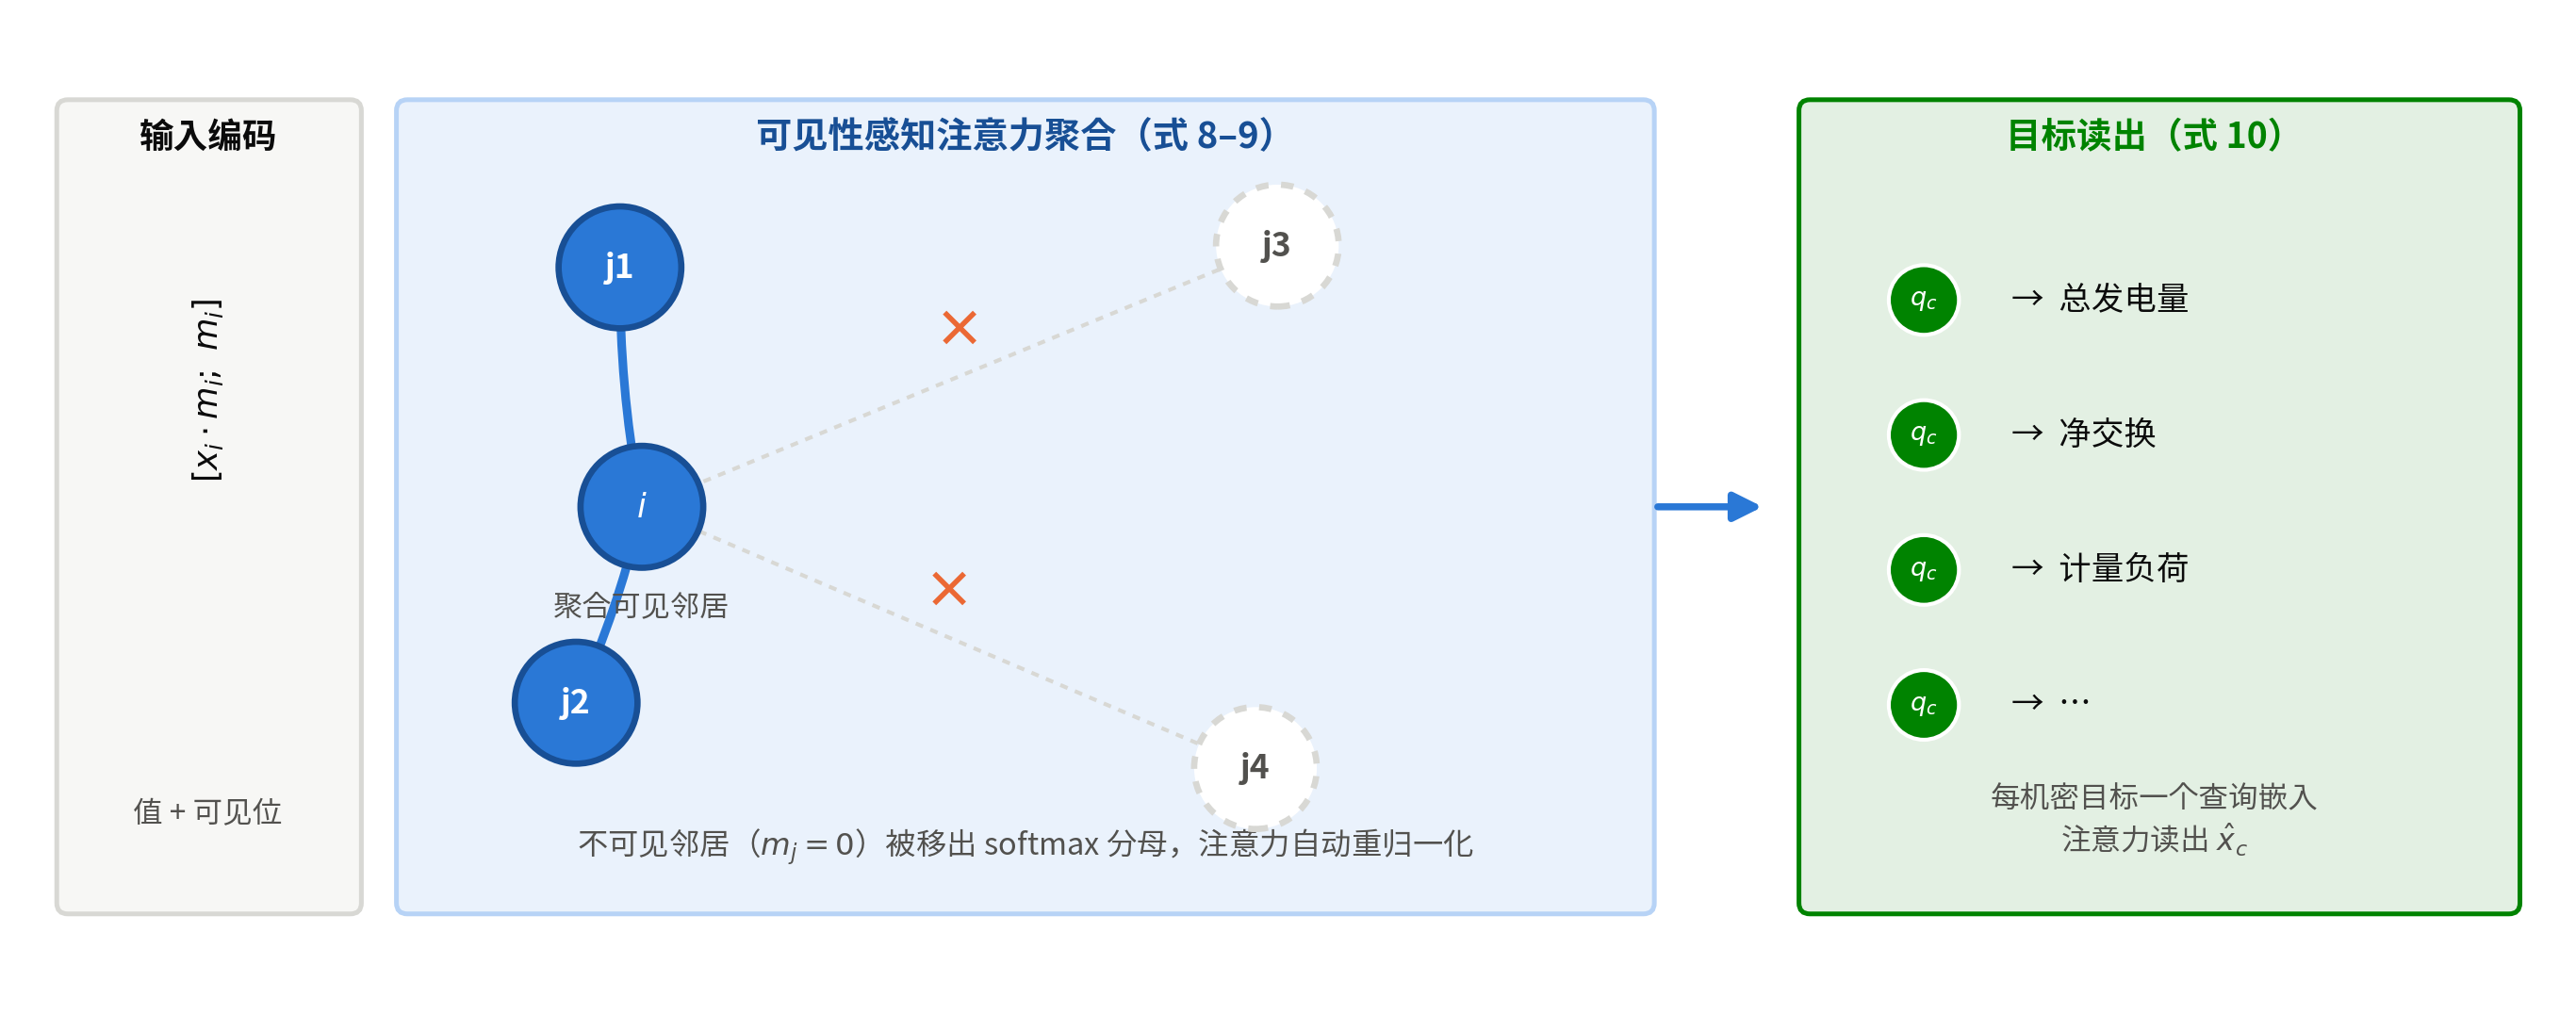
\includegraphics[width=0.99\linewidth]{model_arch_zh.png}}
{\heiti 图 2\quad 子集条件图 oracle 的可见性感知消息传递。节点编码“值 + 可见位”；不可见邻居（$m_j{=}0$）被移出注意力 softmax 的分母，使同一组参数自适应任意可见掩码；每个机密目标由独立查询嵌入注意力读出}
\label{fig:model}
\end{figure}

\subsection{随机子集失活训练}

为使单一 oracle 覆盖任意集合查询，采用\textbf{随机子集失活}联合训练：每个批次独立采样可见集合 $S\sim\pi$，模型在掩码输入下同时回归全部机密字段，
\begin{equation}
\min_{\theta}\ \mathbb{E}_{S\sim\pi}\,\mathbb{E}_{x}\sum_{c\in C}\bigl(f_{\theta}(x\odot m_S,m_S)_c-x_c\bigr)^2 .
\label{eq:oracle}
\end{equation}
掩码分布 $\pi$ 采用两段式采样：先均匀采尺寸 $|S|\sim\mathrm{U}\{1,\dots,|G|\}$，再在该尺寸内均匀采集合。若直接对 $2^{|G|}$ 均匀采样，集合尺寸会集中于 $|G|/2$ 附近，导致小、大集合两端训练不足；两段式采样保证各规模的掩码都被充分覆盖。

单一参数集须在指数多的掩码任务上同时逼近条件期望 $\mathbb{E}[x_c\mid X_S]$，其估计相对重训真值存在两类偏差：一是摊销容量在任务间分配带来的逼近误差，二是方向上系统性\textbf{低估}——oracle 无法对每个 $S$ 专用优化，其精度天然不高于最优响应。后一性质对协议设计反而有利（4.6 节保守性），前一误差由查询时微调闭合。

\subsection{查询时 $K$ 步微调}

对查询集合 $S$，从 oracle 参数 $\theta^{*}$ 出发、仅以 $S$ 的固定掩码继续训练 $K$ 步：
\begin{equation}
\theta_S^{(K)}=\theta^{*}-\eta\sum_{t=1}^{K}\nabla_{\theta}\mathcal{L}_S(\theta_S^{(t-1)}),\qquad
\hat v_c^{(K)}(S)=\max\bigl(0,R^2_{\mathrm{test}}(f_{\theta_S^{(K)}})\bigr),
\label{eq:finetune}
\end{equation}
$\mathcal{L}_S$ 为式 (\ref{eq:oracle}) 在固定 $m_S$ 下的损失。这一暖启动微调把 oracle 的通用表示快速特化到目标集合：$K$ 步成本远低于冷启动重训（后者需数百轮），而实验表明 $K$ 与保真度单调正相关（5.2 节）。本文取 $K=200$ 作为工作点，每集合约 3 秒，相对完整重训将成本压缩两个数量级以上。查询语义上，一次“查询”本身就是在测试集上实测 $R^2$，只是被测模型为（微调后的）oracle 而非专用重训模型。

\subsection{应用于协同发现：扫描—认证协议}

$k$ 阶协同候选空间为 $\binom{n}{k}$（$k=3$ 时 13244），重训穷举不可行、纯估计又不可信。借助秒级 oracle，本文以“扫描 + 认证”闭环解决这一矛盾，流程见算法 1。

\begin{algorithm}[htbp]
\caption{$k$ 阶协同扫描—认证协议}
\label{alg:scan}
\begin{algorithmic}[1]
\Require oracle 参数 $\theta^{*}$；低阶重训真值 $\{v_c(T'):|T'|<k\}$；预算 $B_{\mathrm{top}},B_{\mathrm{rand}}$；显著阈值 $\delta$
\Ensure 认证的 $k$ 阶协同超边 $E_k$ 及协议可靠性检验量
\For{每个候选 $T\in\binom{F}{k}$}\Comment{扫描：秒级}
  \State 按式 (\ref{eq:finetune}) 微调 $K$ 步并前向，得 $\hat v_c(T)$
  \State 结合低阶真值按式 (\ref{eq:synk}) 计算估计协同 $\widehat{\mathrm{syn}}_k^c(T)$
\EndFor
\State 按 $\widehat{\mathrm{syn}}_k$ 对全体候选排序
\State 取估计 top-$B_{\mathrm{top}}$ 候选，另均匀随机抽取 $B_{\mathrm{rand}}$ 个对照
\For{每个被选 $T$}\Comment{认证：重训}
  \State 按专用攻击者协议从头重训，得真值 $\mathrm{syn}_k^c(T)$
\EndFor
\State 检验：(a) 估计与真值的 Spearman 排序一致性；(b) 估计是否系统性不高于真值（保守性）；(c) 对照组中 $\mathrm{syn}_k>\delta$ 的比例（稀疏性）
\State \Return $E_k=\{T:\mathrm{syn}_k^c(T)>\delta\}$ 及检验量
\end{algorithmic}
\end{algorithm}

协议可靠性建立在两个\textbf{可检验}前提上。\textbf{排序一致性}：估计排序需与真值排序足够相关，top 筛选才能覆盖真强项。\textbf{保守性}：若估计系统性低估（4.4 节的摊销残差方向），则一个在低估口径下仍突出的候选在真值下只会更强，筛选不漏针。两者均在认证样本上直接检验（算法 1 第 11 行），而非作为假设接受。随机对照组承担双重职能：控制“top 组数字被选择偏差抬高”的风险，并独立测量高阶协同在整个空间的背景稀疏率。扫描成本为 $\binom{n}{k}\times O(K)$ 梯度步（$k=3$ 时约 11 GPU 时），认证成本 $(B_{\mathrm{top}}+B_{\mathrm{rand}})$ 次重训、与 $\binom{n}{k}$ 解耦。向更高阶推广时，可利用协同稀疏性做先验式剪枝：仿频繁项集挖掘，$k{+}1$ 阶候选仅在已认证的强 $k$ 阶超集中生成。

\section{\heiti 实验}

实验围绕四个研究问题：\textbf{RQ1}（oracle 保真度与成本）——oracle 能否以秒级成本忠实逼近重训真值？\textbf{RQ2}（消融）——图结构与微调各自贡献多少，图相对多层感知机的收益在哪？\textbf{RQ3}（应用一）——协同泄露是否真实存在，既有置零口径是否失效？\textbf{RQ4}（应用二）——扫描—认证协议能否在 13244 个三元组中可靠定位真三阶协同？

\subsection{实验设置}

\textbf{数据集}。PJM 电网 2025 年小时级公开运行数据，清洗对齐后 $n=44$ 字段、全年样本。机密字段 $|C|=12$。数据按 7:3 划分（切分种子 42），重训统一种子 0，oracle 另做 3 种子稳定性复核。

\textbf{模型与协议}。字段相关图：五度量融合、$\tau=0.15$、$k_{\min}=8$。oracle 与专用攻击者同构（式 (\ref{eq:enc})--(\ref{eq:readout})），隐藏维 64、Adam、学习率 $10^{-3}$、权重衰减 $5\times10^{-4}$、批大小 128；专用攻击者至多 500 轮早停（耐心 150），oracle 微调 $K\in\{0,10,50,200\}$。图 oracle 与其多层感知机对照使用相同掩码序列、批次顺序与优化器，保证一切对比在同等优化预算下进行。

\textbf{真值库与指标}。累计构建重训真值 1437 条评测记录（1431 个不同字段集合、17172 条逐机密字段真值）：全部 44 个单字段、全部 $\binom{44}{2}=946$ 个字段对、397 个认证三元组（top 197 + 随机 200）、50 个宽尺寸随机集合（规模 1--44，分 5 带各 10 个）。指标为逐机密字段 $R^2$、oracle 相对真值的平均绝对误差（MAE）、集合排序 Spearman 相关系数与每集合评估耗时。

\subsection{RQ1：oracle 保真度与成本}

这是本文最核心的实验。图 3 直接对比 oracle 逐条估计 $\hat v_c(S)$ 与重训真值 $v_c(S)$（17172 条逐机密字段记录）。不微调（$K{=}0$）时散点已沿对角线分布、整体排序 Spearman 达 0.90，但系统性位于对角线\textbf{下方}——印证 4.4 节所述摊销 oracle 的系统性低估；微调 200 步后散点显著收紧至对角线附近，池化 MAE 降至 0.039、排序 Spearman 升至 0.95。这一“低估但可微调闭合”的行为模式正是扫描—认证协议成立的经验基础。

\begin{figure}[htbp]
\centering
\centerline{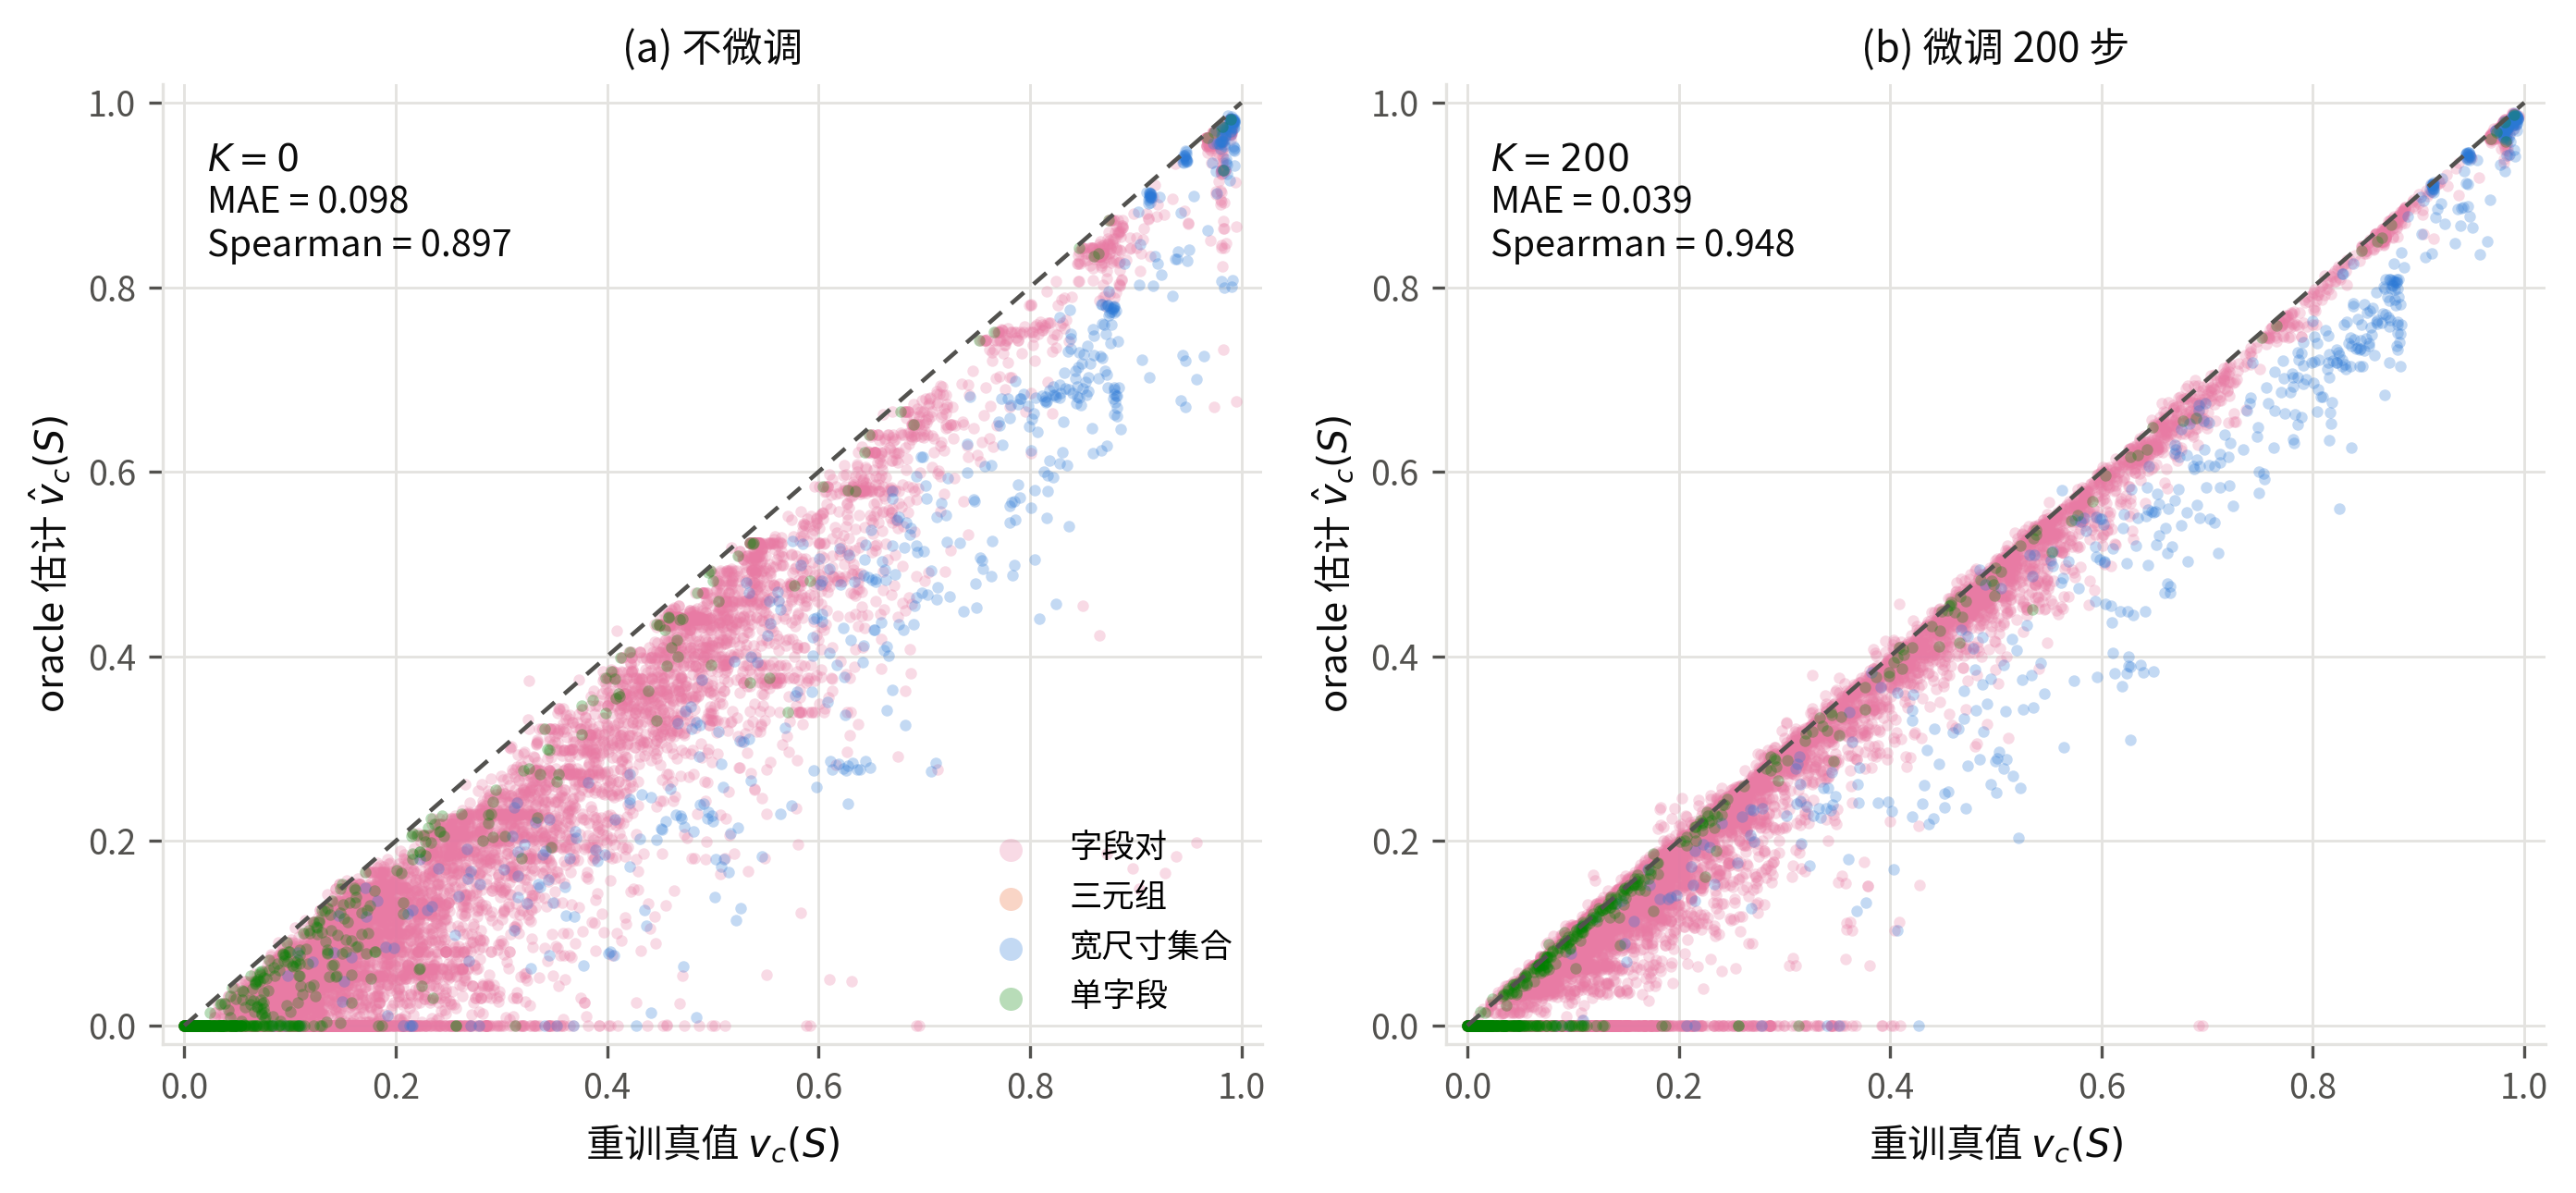
\includegraphics[width=0.99\linewidth]{oracle_calibration_zh.png}}
{\heiti 图 3\quad oracle 估计与重训真值的校准散点（17172 条逐机密字段记录，虚线为 $y=x$）：(a) 不微调，估计系统性偏低（点在对角线下方）；(b) 微调 200 步后估计紧贴对角线。颜色区分集合类别}
\label{fig:calib}
\end{figure}

表 1 按集合类别给出保真度随微调步数的收敛。三点结论：(1) 摊销估计的\textbf{排序信息在 $K{=}0$ 已可用}——宽尺寸集合排序 Spearman 已达 0.975，字段对 0.962，oracle 单次前向即可胜任“哪些集合更危险”的粗排，这是扫描协议的成本下界；(2) 微调\textbf{单调闭合绝对误差}——$K$ 由 0 增至 200，宽尺寸集合 MAE 由 0.136 降至 0.078，字段对由 0.081 降至 0.035，三元组由 0.138 降至 0.044，三元组排序由 0.846 升至 0.973；(3) 成本压缩两个数量级——$K{=}200$ 每集合约 3.1 秒，而完整重训需分钟级，13244 个三元组全扫描因此从不可行变为约 11 GPU 时。

\begin{table}[htbp]
\centering {\heiti 表 1\quad 图 oracle 保真度随微调步数 $K$ 的变化（相对重训真值）}
\vspace {1mm}
\begin{center}
\zihao{5-}
\begin{tabular}{lccccc}
\toprule
集合类别 & MAE ($K{=}0$) & MAE ($K{=}200$) & Spr. ($K{=}0$) & Spr. ($K{=}200$) & 耗时/秒 ($K{=}200$) \\
\midrule
单字段（44 个）        & 0.040 & ---   & 0.976 & ---   & --- \\
字段对（946 个）       & 0.081 & 0.035 & 0.962 & 0.988 & 3.0 \\
三元组（397 个）       & 0.138 & 0.044 & 0.846 & 0.973 & 3.1 \\
宽尺寸集合（50 个）    & 0.136 & 0.078 & 0.975 & 0.985 & 3.1 \\
\bottomrule
\end{tabular}
\label{tab:fidelity}
\end{center}
\end{table}

图 4(a) 进一步展示 oracle 在\textbf{各集合规模}上都紧贴重训攻击上限：oracle 估计的平均 $R^2$ 曲线与重训真值曲线在 1--44 全规模高度贴合，逐带 MAE 均在 0.03--0.11。图 4(b) 给出微调的成本—保真度权衡：MAE 随耗时快速下降并在 $K{=}50$（约 0.8 秒）后进入平台，说明即便更激进地压缩预算，排序质量也已足够；实际中可按“先小 $K$ 粗扫、对候选大 $K$ 精认证”分层配置。

\begin{figure}[htbp]
\centering
\subfigure[oracle 估计紧贴逐规模重训上限]{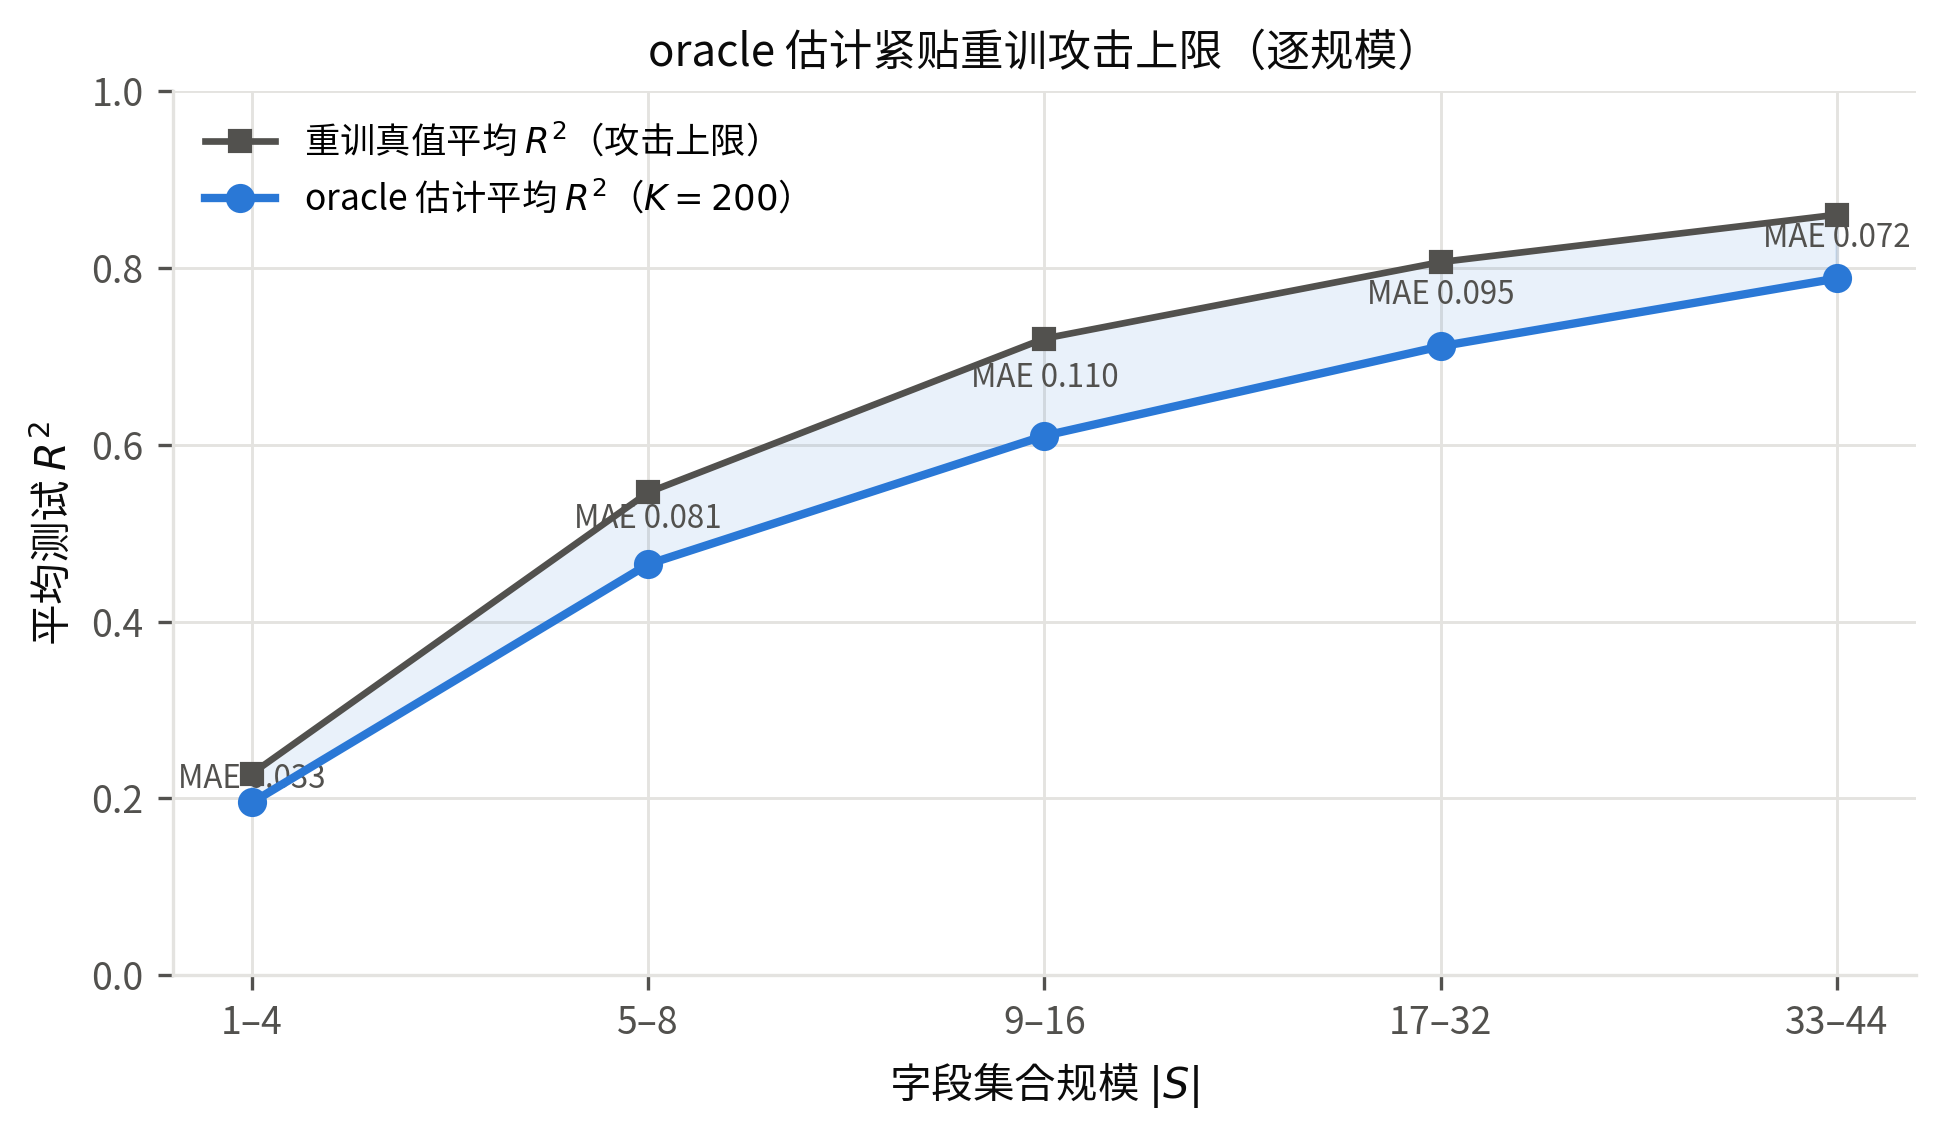
\includegraphics[width=0.485\linewidth]{fidelity_by_size_zh.png}}
\subfigure[成本—保真度权衡与种子稳健性]{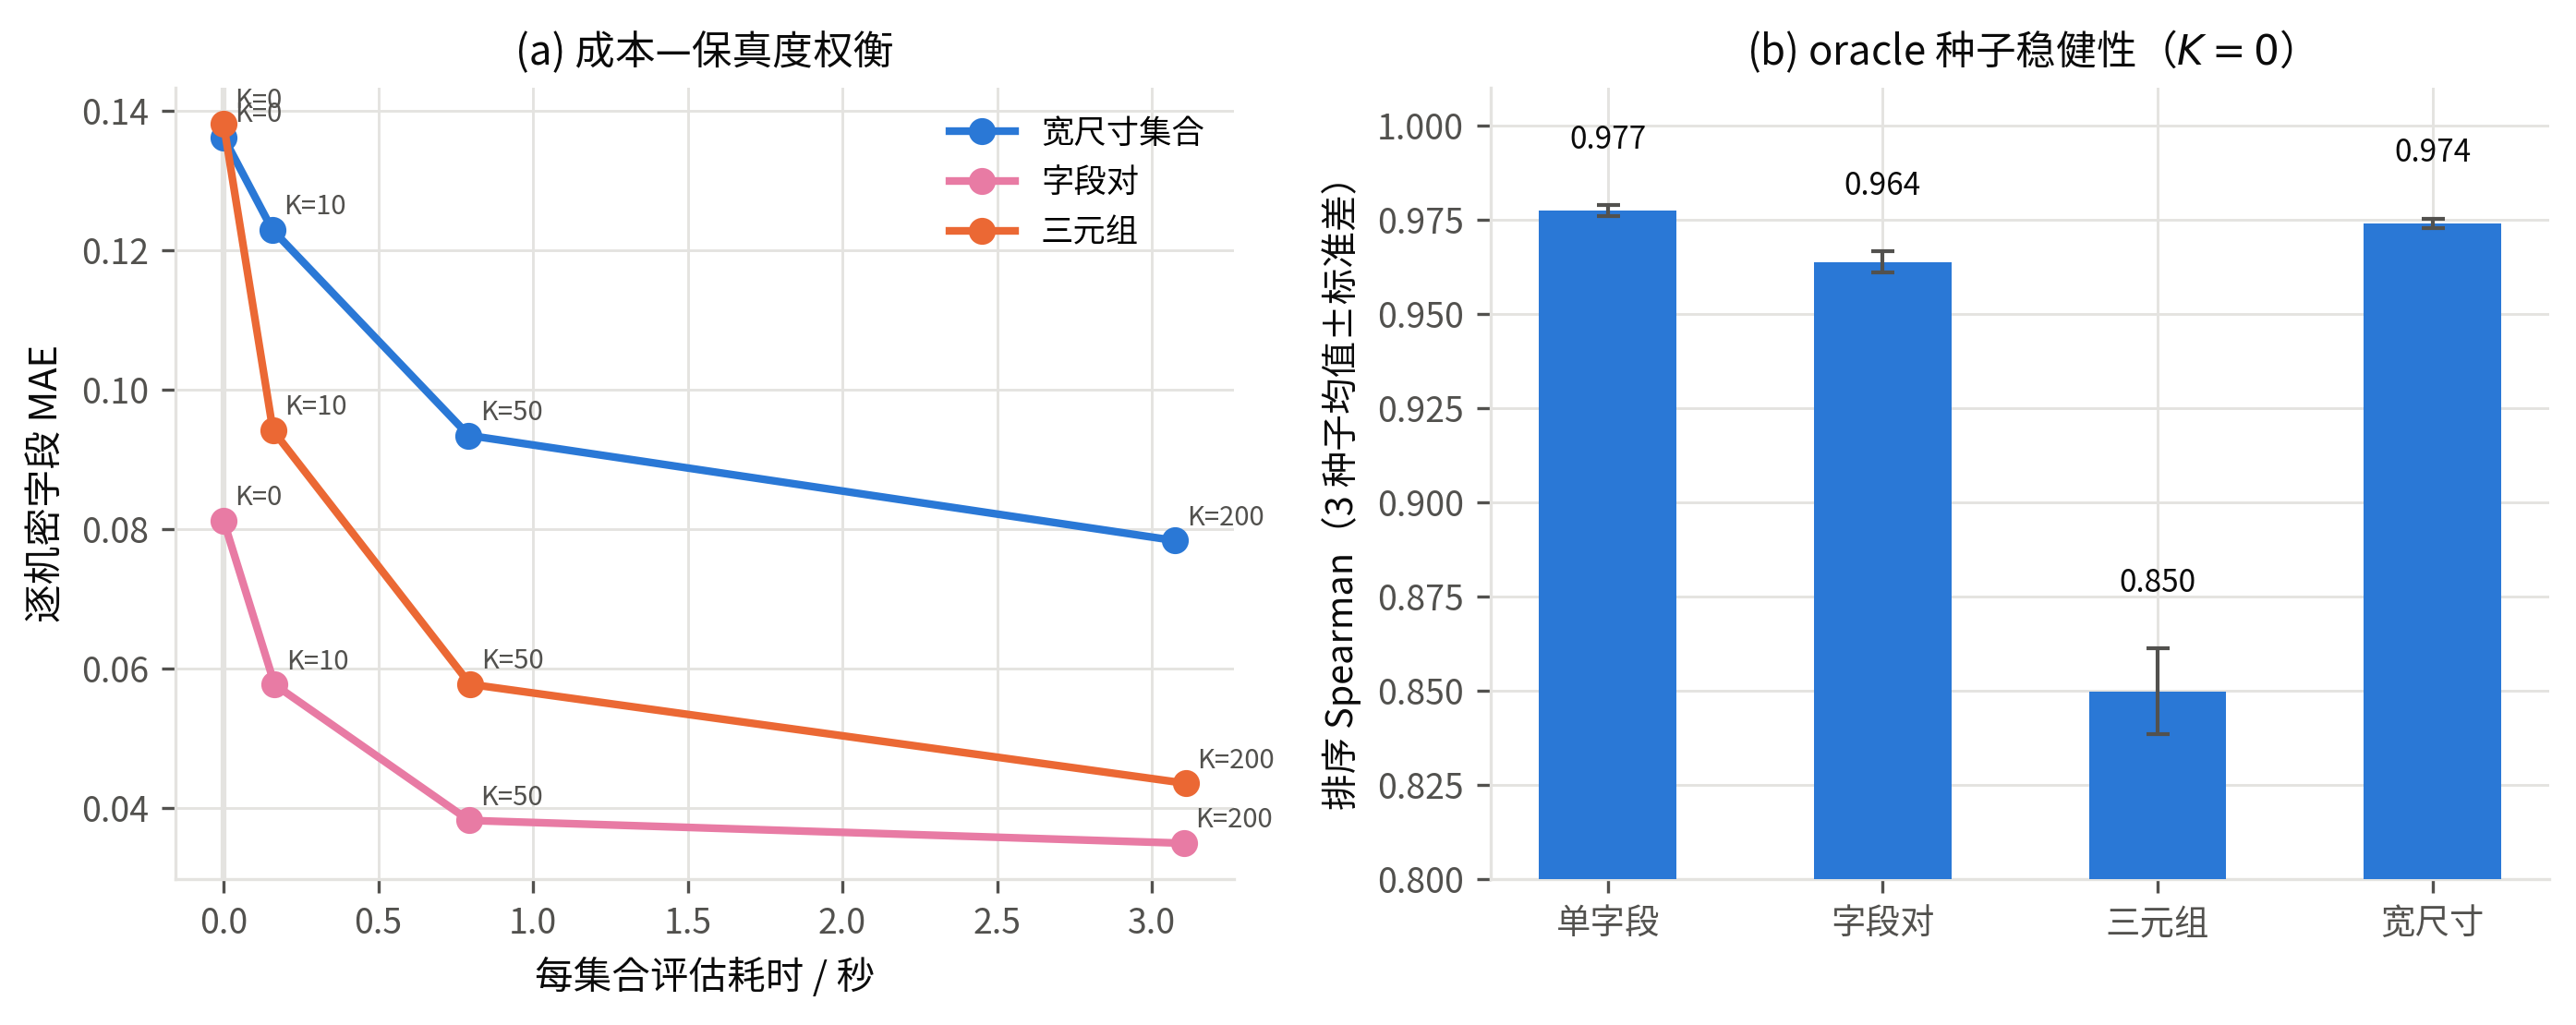
\includegraphics[width=0.495\linewidth]{cost_seed_zh.png}}
{\heiti 图 4\quad (a) oracle（$K{=}200$）估计平均 $R^2$ 与重训攻击上限在各规模带上高度贴合；(b) 左：MAE 随每集合耗时下降并在 $K{=}50$ 后进入平台；右：3 个 oracle 种子的排序 Spearman 稳定（误差棒为标准差）}
\label{fig:cost}
\end{figure}

图 4(b) 右侧的种子稳健性检验表明结论并非单一 checkpoint 偶然：3 个独立 oracle 种子在各集合类别的排序 Spearman 标准差均在 0.001--0.011，单/对/宽尺寸稳定在 0.96--0.98，三元组为 0.850$\pm$0.011。\textbf{RQ1 结论}：子集条件图 oracle 能以约 3 秒/集合的成本忠实逼近重训真值（微调后 MAE 0.039、排序 Spearman 0.95），且低估可预测、可微调闭合、跨种子稳定，为指数空间的敏感度检索提供了可行的估计层。

\subsection{RQ2：消融——图结构与微调的贡献}

\textbf{微调的贡献}已由表 1 与图 5(b) 充分展示（MAE 随 $K$ 单调下降 40\%--68\%）。此处聚焦\textbf{图结构相对无结构基线的收益}。图 5 在 50 个宽尺寸随机集合上对每个集合分别从头重训图攻击者与多层感知机攻击者（协议完全一致）：图结构在 5 字段及以上的所有规模带平均 $R^2$ 一致更高（5--8 带 +0.023，超过图模型显著标尺），逐集合胜率随规模从 20\%单调升至 90\%；仅在极小集合（1--4 字段）无优势——此时图中大量不可见节点使消息传递退化，无结构的多层感知机更直接。此外两种结构互补：逐机密字段取较优者可再获 0.005--0.017 的包络增益，这也是本文以 best-of-struct 近似 $\sup$ 的依据。

需要如实指出图结构收益的边界：在\textbf{摊销 oracle} 这一角色上，同等优化步数下无结构的多层感知机估计器在绝对误差上仍具竞争力，图 oracle 的优势体现为排序保真度已足够支撑扫描协议（Spearman $\ge$0.97），而非逐点精度全面领先。这与关系归纳偏置的一般规律一致\upcite{battaglia2018relational,grinsztajn2022tabular}：专用推断的依赖结构与相关图对齐，图先验获益；对任意掩码的摊销回归更接近无结构表格学习，红利有限。\textbf{RQ2 结论}：图结构的收益集中于中大规模集合的专用推断与结构互补，宜作攻击上限的结构之一；摊销扫描则由 oracle 承担吞吐，两者按角色分工。

\begin{figure}[htbp]
\centering
\centerline{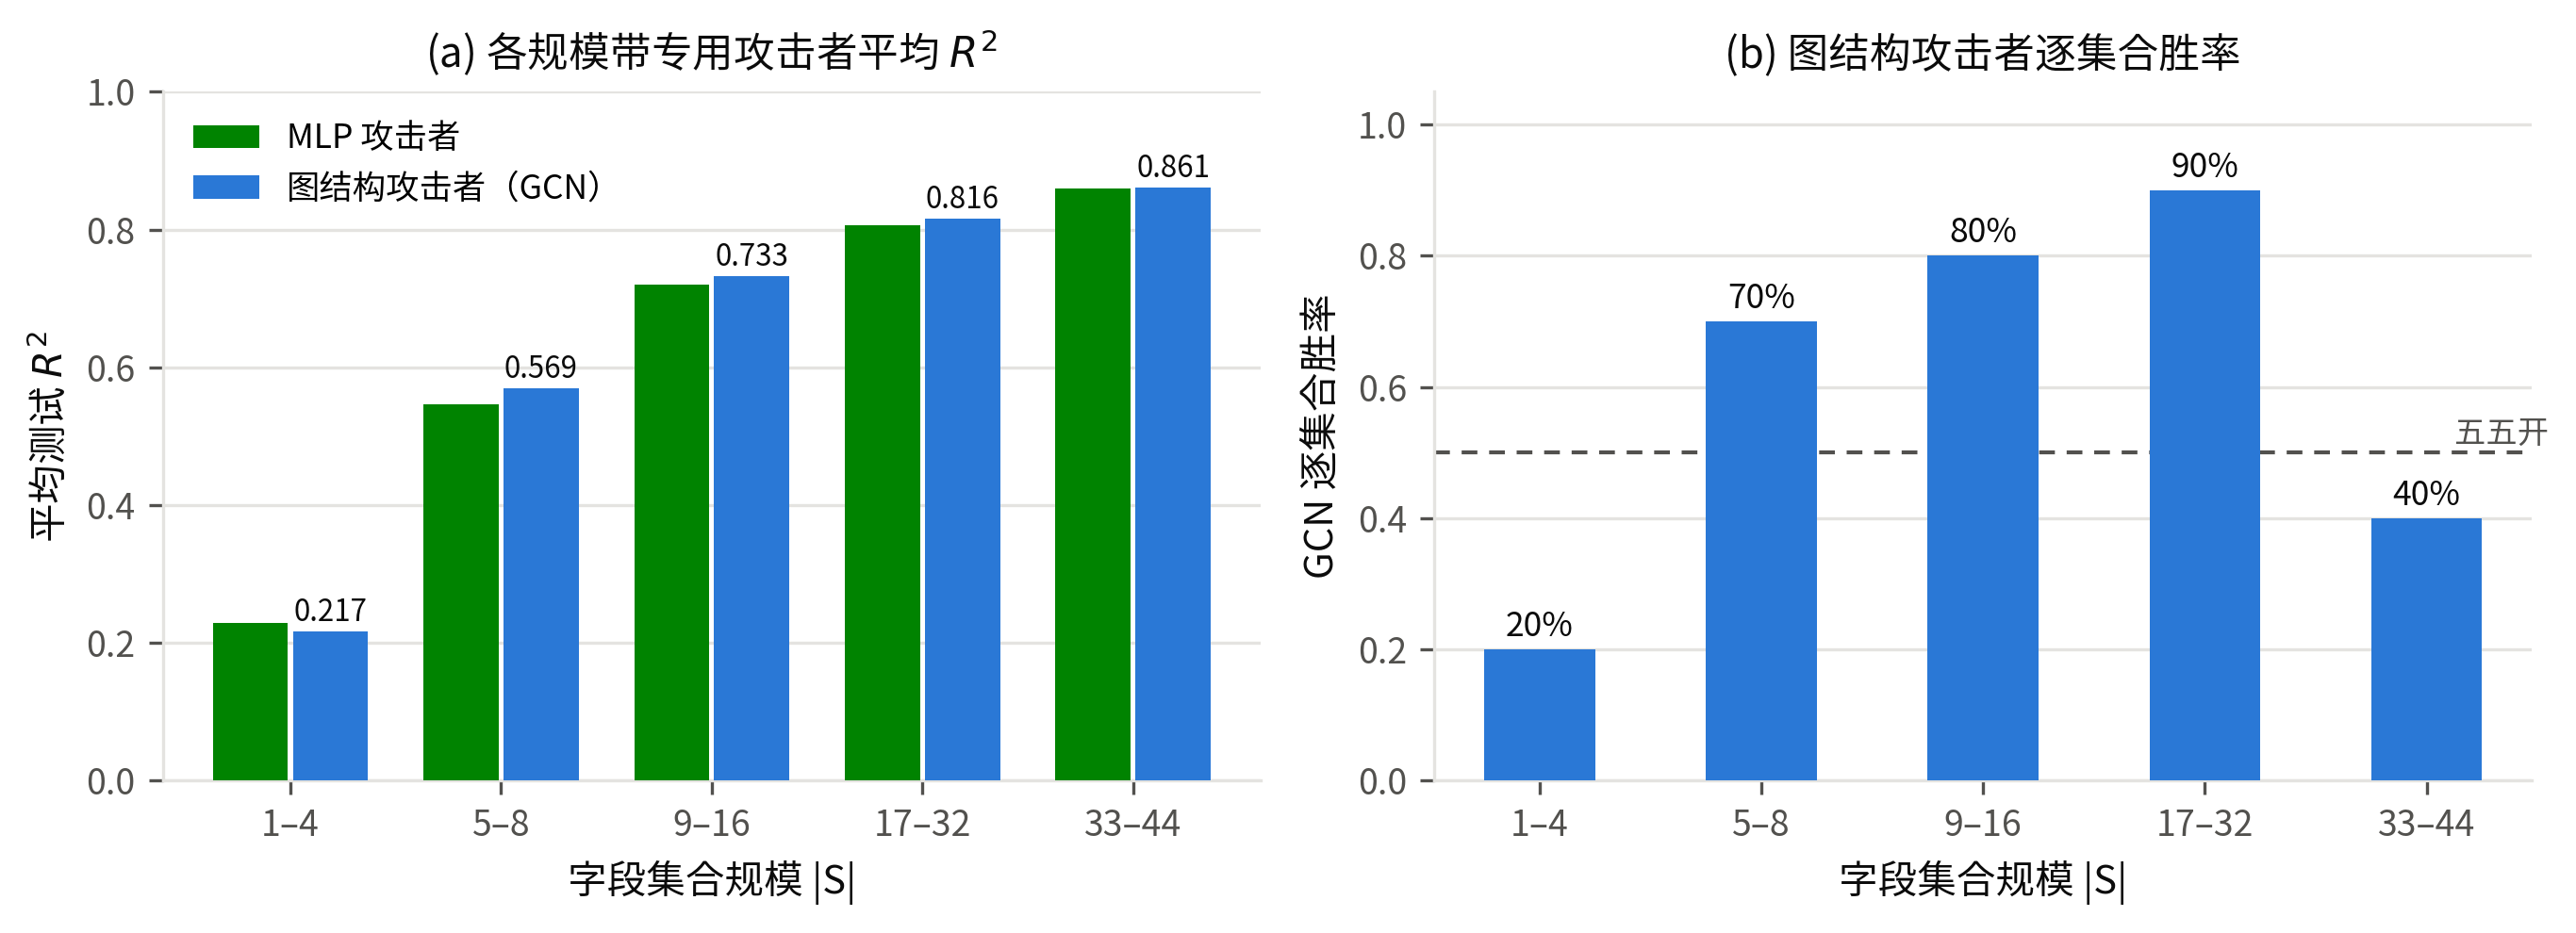
\includegraphics[width=0.99\linewidth]{attacker_compare_zh.png}}
{\heiti 图 5\quad 图结构与多层感知机专用推断模型的消融（50 个宽尺寸随机集合，逐集合重训）：(a) 各规模带平均测试 $R^2$；(b) 图模型逐集合胜率随集合规模从 20\%升至 90\%}
\label{fig:ablation}
\end{figure}

\subsection{RQ3：应用一——任意集合敏感度与二阶协同图}

有了秒级 oracle，任意集合的敏感度评估成为查表式操作。本节展示其首个价值：低成本构建完整的二阶协同图。对全部 946 个字段对重训得 $G_{\mathrm{syn}}$ 的完整真值（图 6 热力图），显著协同高度集中于少数字段对；表 2 列出最强者，均共享清晰物理机制——各类燃料的“出力 + 占比”对合体可精确恢复总发电量（总发电 $=$ 出力 $\div$ 占比），两字段各携比值一端，合体才构成完整方程。风电对协同增量达 0.765；太阳能出力单独 $R^2$ 仅 0.006，却参与 0.596 的协同。

\begin{observation}[单字段评分的不适定性]
表 2 中字段在任何单字段评分下均属低风险（$v_c\le0.29$），但其两两组合泄露达 0.70--0.96。不存在仅依赖单字段分数的单调聚合规则能同时正确刻画“太阳能出力单独共享安全”与“其与占比合体高危”——前者要求其分数低、后者要求其分数高。敏感度必须定义在集合上。
\end{observation}

\begin{figure}[htbp]
\centering
\centerline{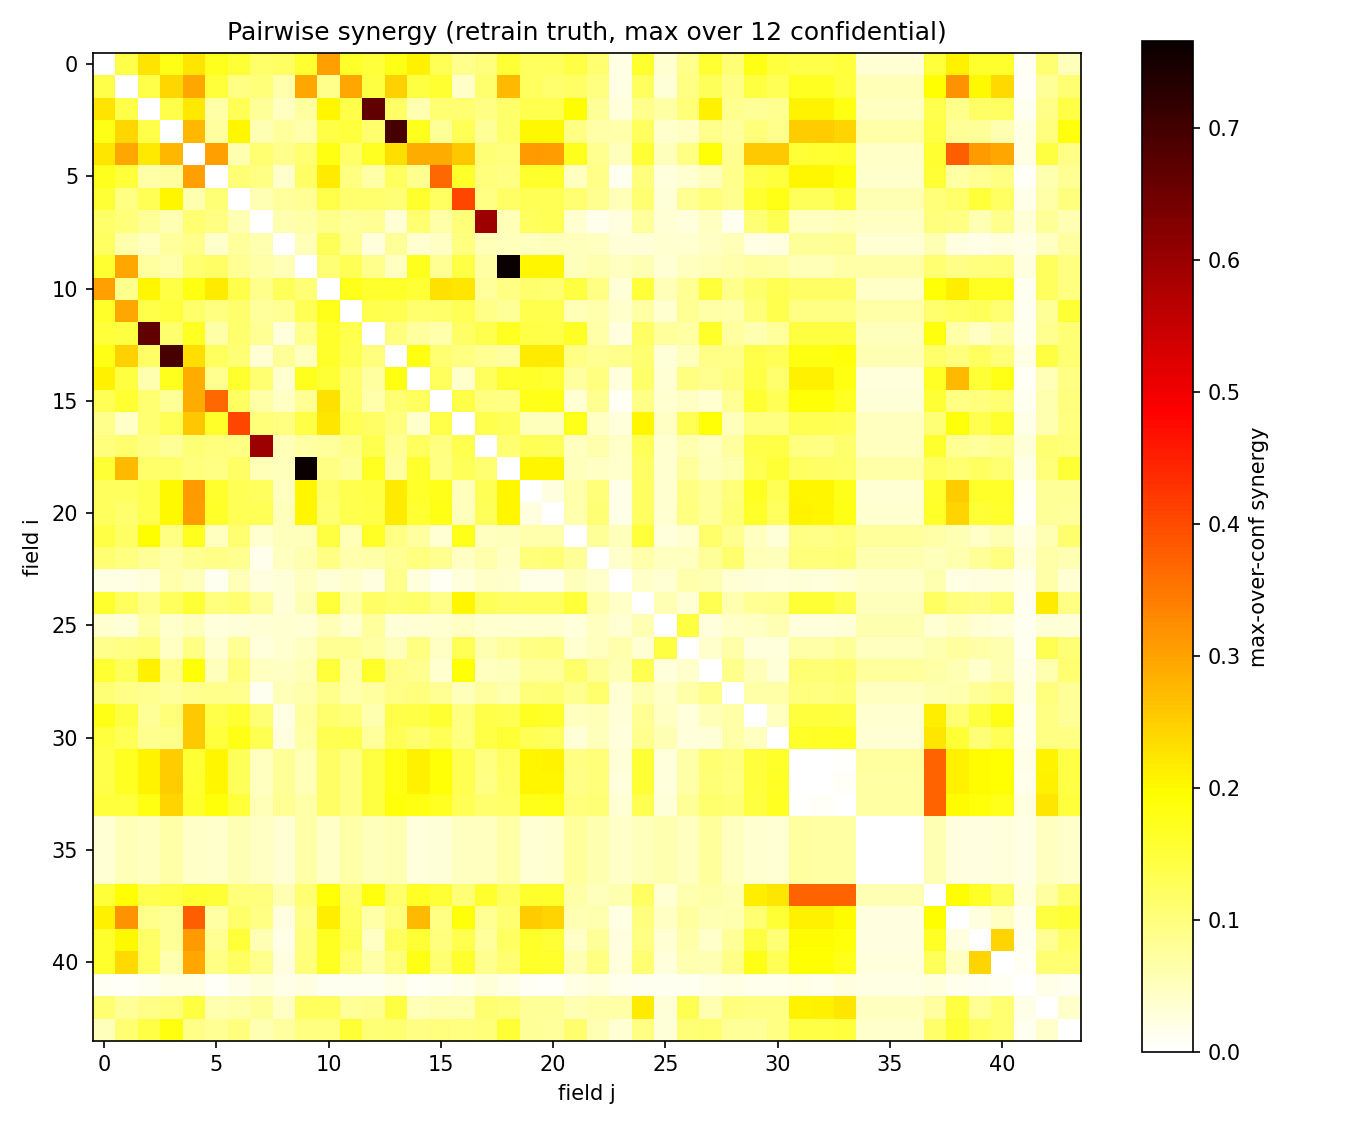
\includegraphics[width=0.66\linewidth]{synergy2_heatmap.png}}
{\heiti 图 6\quad 二阶协同图 $G_{\mathrm{syn}}$ 邻接矩阵热力图（946 个字段对全部重训，对 12 个机密字段取最大值）。显著协同（深色）集中于少数“出力—占比”字段对，呈明显稀疏结构}
\label{fig:heatmap}
\end{figure}

\begin{table}[htbp]
\centering {\heiti 表 2\quad 最强二阶协同对（全部为重训真值）}
\vspace {1mm}
\begin{center}
\zihao{5-}
\begin{tabular}{llcccc}
\toprule
字段对 $(i,j)$ & 机密目标 $c$ & $v_c(\{i\})$ & $v_c(\{j\})$ & $v_c(\{i,j\})$ & $\mathrm{syn}_2^c$ \\
\midrule
风电出力 + 风电占比     & 总发电量 & 0.064 & 0.162 & 0.928 & \textbf{0.765} \\
多燃料出力 + 多燃料占比 & 总发电量 & 0.201 & 0.078 & 0.897 & 0.696 \\
水电出力 + 水电占比     & 总发电量 & 0.292 & 0.135 & 0.957 & 0.665 \\
太阳能出力 + 太阳能占比 & 总发电量 & 0.006 & 0.099 & 0.695 & 0.596 \\
\bottomrule
\end{tabular}
\label{tab:syn2}
\end{center}
\end{table}

\textbf{置零口径系统性失效}。在同一批字段对上按 3.4 节计算置零协同并与重训真值对比：置零均值 0.012、重训均值 0.041，系统性低估 3.4 倍；两者排序 Spearman 仅 0.351。即置零既低估绝对量又排不对顺序，依赖它的评估会漏报几乎全部头部协同，原因正是其分布外伪影与无最优响应。\textbf{RQ3 结论}：协同泄露是物理级现实，单字段评分与置零口径均不适定，一切协同数值必须来自重训认证。

\subsection{RQ4：应用二——三阶协同的扫描与认证}

以 $K{=}200$ oracle 执行算法 1（$k=3$，$B_{\mathrm{top}}=B_{\mathrm{rand}}=200$，$\delta=0.10$），扫描全部 13244 个三元组、认证 397 个（top 去重后 197），认证记录按（三元组，机密字段）展开共 4764 条，结果见图 7。

\begin{figure}[htbp]
\centering
\centerline{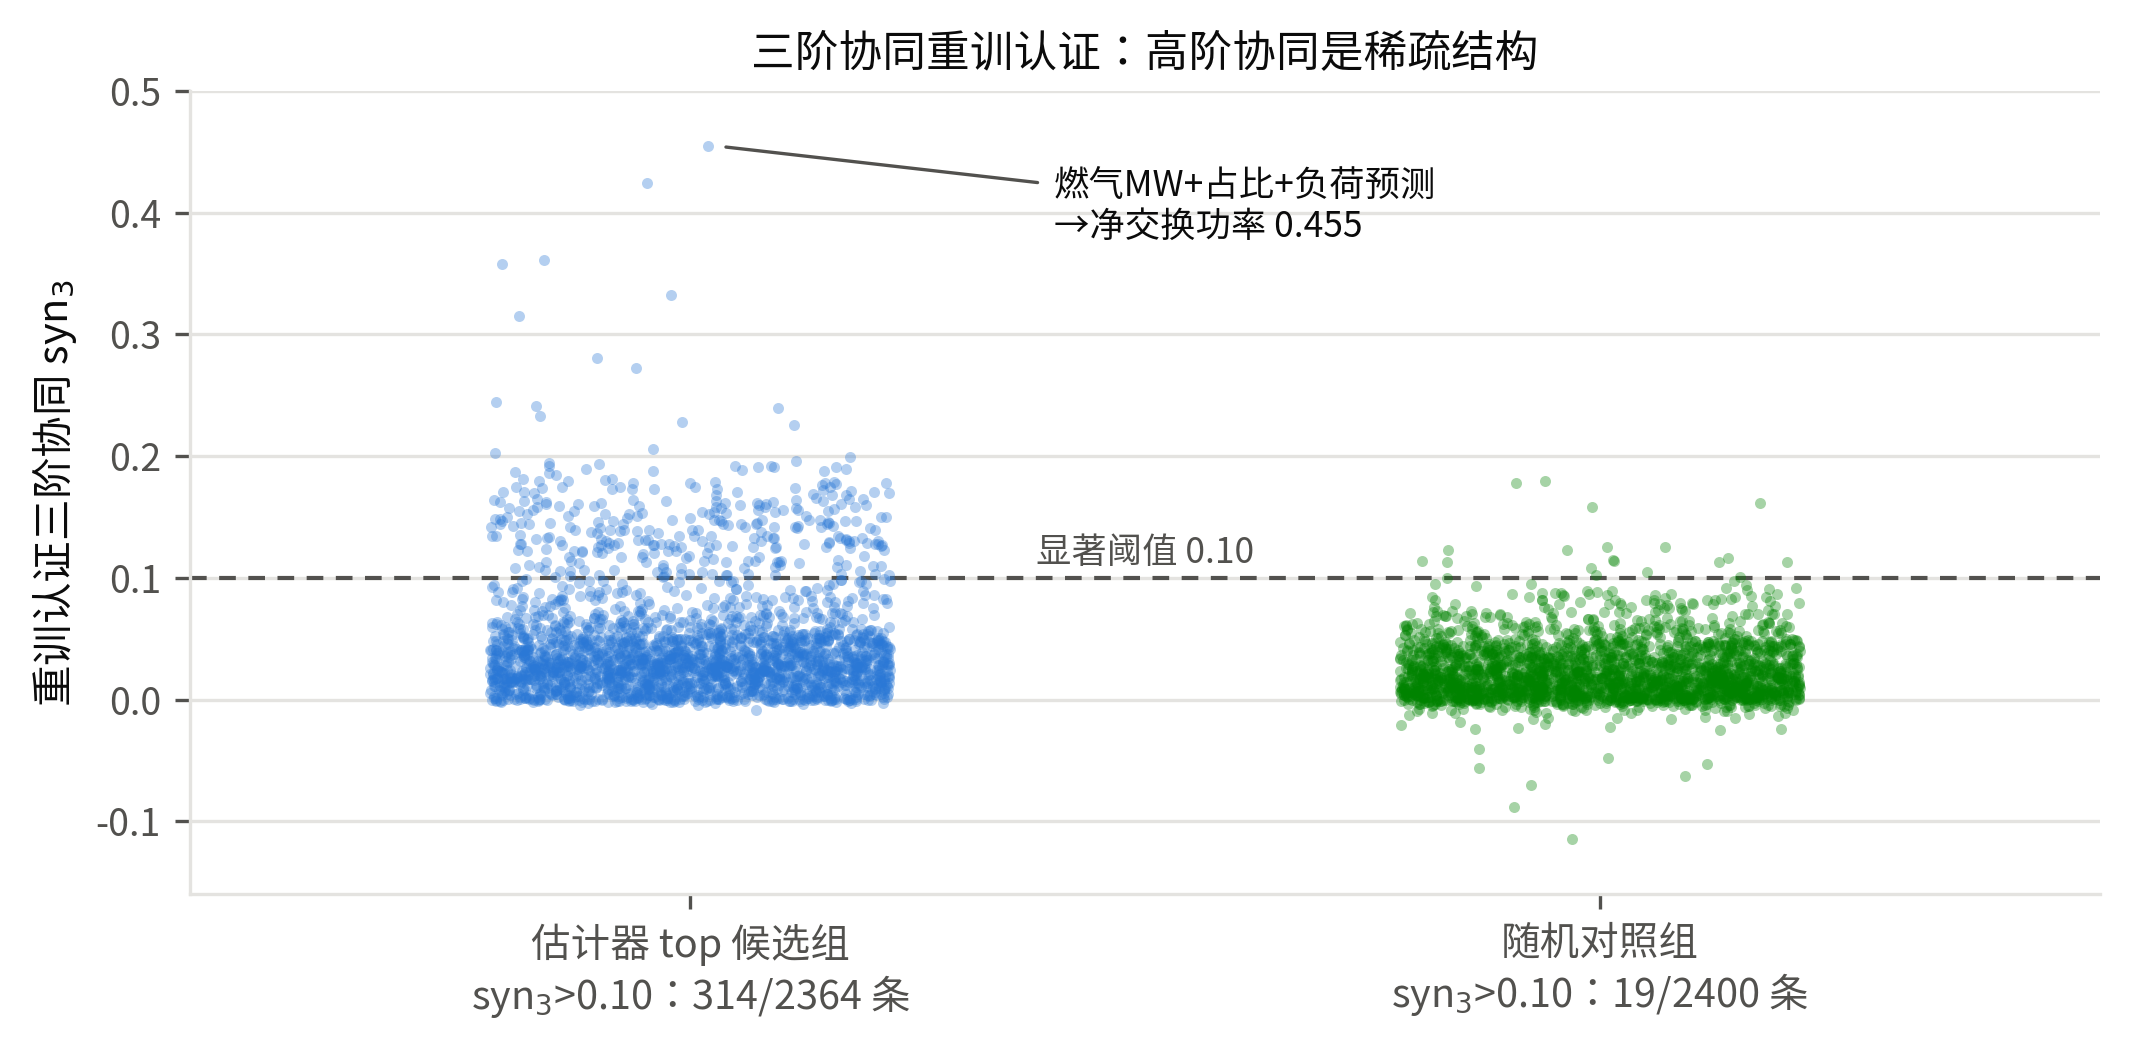
\includegraphics[width=0.82\linewidth]{triple_certify_zh.png}}
{\heiti 图 7\quad 三阶协同重训认证。top 候选组 2364 条认证记录中 314 条超过显著阈值 $\delta{=}0.10$；随机对照组 2400 条中仅 19 条，中位数 0.018 处于噪声底附近}
\label{fig:triple}
\end{figure}

\textbf{协议检验通过}：(a) 认证样本上估计与真值 Spearman 相关 0.795，top 筛选有效覆盖真强项；(b) 保守性成立——估计系统性不高于真值（最强项估计 0.421、认证 0.455），与 4.4 节分析一致，筛选不漏针；(c) 稀疏性——随机对照组阳性率仅 19/2400（0.8\%）、中位数 0.018 处于噪声底。\textbf{真不可约三阶协同存在且物理可解释}：最强者“燃气出力 + 燃气占比 + 最新负荷预测 $\to$ 净交换功率”$\mathrm{syn}_3=0.455$，而其三个二元子集最优仅 0.24--0.28；机制为净交换 $=$ 发电 $-$ 负荷，恢复发电需“出力+占比”两字段、恢复负荷需“负荷预测”一字段，三者缺一不可，是超越一切二阶分析的三方合谋泄露；燃煤、核电、水电、风电的同构三元组认证值 0.24--0.42，构成 $H_{\mathrm{syn}}$ 中结构一致的一族超边。头部协同集中于“低阶强协同 + 一个补全字段”的模式，而随机三元组几乎无协同，这一稀疏性支持 4.6 节的先验式剪枝。\textbf{RQ4 结论}：扫描—认证协议能在指数级组合空间中可靠、保守地定位并认证真高阶协同。

\section{\heiti 讨论}

\textbf{图结构的适用边界}。本文将图结构收益定位于专用推断通道（RQ2），并如实指出其在摊销 oracle 角色上的有限性。按角色分工——图结构负责攻击上限与结构组织、摊销估计负责扫描吞吐——是务实选择，也与关系归纳偏置的适用规律相符。

\textbf{可迁移性}。oracle 参数由共享的消息、注意力与读出函数构成，与字段数量、顺序及身份解耦，节点仅需去身份化输入（值与可见位）。这意味着面对字段集不同的另一电网系统，图 oracle 在结构上支持直接迁移或少样本适配，而多层感知机首层与字段维度绑定、无法跨系统复用。在 IEEE 标准算例上开展跨系统迁移并与 IGNN 正面对比，是最自然的延伸；本文以分析性论证给出该方向，实验验证留作未来工作。

\textbf{可扩展性与低阶稀疏猜想}。RQ4 的稀疏性提示 $v_c(\cdot)$ 可能具有布尔函数意义上的低度数近似结构\upcite{odonnell2014boolean}：若 $v_c$ 能由单字段、显著二阶与三阶项良好重构，则任意集合评估从 $2^n$ 塌缩为 $O(n^3)$ 个已认证系数的查询与组合，且本文已备有 50 个宽尺寸随机集合真值作为独立检验集。结合 4.6 节的先验式剪枝，框架有望推广到字段数显著更多的系统。

\textbf{局限}。(1) 协同显著阈值 $\delta=0.10$ 是基于噪声底的经验选择；(2) 三阶 top 候选来自估计器扫描，尽管保守性检验通过，稀疏性结论仍以随机对照组为准；(3) $\sup$ 语义以两种结构的 best-of-struct 近似，真实攻击者模型族更大，故本文数值应理解为攻击风险的\textbf{下界证词}——真实风险只会更高，这使泄露警示更稳健，但对“安全”的判定需保留余量。

\section{\heiti 结论}

本文针对电网数据共享中的推断泄露，指出单字段敏感度评分无法刻画“单看安全、合体泄露”的协同效应，将敏感度升维为任意集合上的集合函数 $v_c(S)$，并以此为出发点提出本文核心——子集条件图 oracle：通过可见性感知消息传递与随机子集失活训练，一次训练即可对任意可见集合秒级估计敏感度，配合 $K$ 步查询微调将单集合评估成本较完整重训压缩两个数量级（微调后 MAE 0.039、排序 Spearman 0.95、约 3 秒/集合），且低估可预测、跨种子稳定。基于该 oracle 的“扫描—认证”协议在 13244 个三元组的组合空间中可靠、保守地发现真不可约三阶协同（估计—认证排序相关 0.795），产出了完整的二阶协同图与三阶协同超图，最强协同均具清晰物理机制且高阶协同被证明稀疏。实验同时否定了置零口径（低估 3.4 倍、排序相关 0.351），确立“估计只用于筛选、结论以重训证书落地”的测量纪律。未来工作将沿低阶稀疏重构与跨系统迁移两个方向推进，以将框架扩展到更大规模的系统并正面检验图结构参数迁移的价值。

%%%%%%%%%%%%%%%%%%%%%%%%%%%%%%%%%
\vspace {10mm}
\centerline
{\zihao{5}\textsf{参~考~文~献}}
\zihao{5-} \addtolength{\itemsep}{-1em}
\vspace {1.5mm}
\bibliographystyle{gbt7714-numerical}
\bibliography{ref.bib}

\end{document}
